\documentclass[12pt]{article} 
\usepackage{times}
\usepackage{graphicx}
\usepackage{amssymb}
\usepackage{url,hyperref}
\usepackage{cite}
\usepackage{algorithm}
\usepackage{algorithmic}
\input{spanishAlgorithmic}


\begin{document}

\title{\textbf{Implementaci\'on de Risk con algoritmo de Minimax.}}
\author{Prieto Larios, Estefan\'ia,$^{\spadesuit}$\\
Galicia Mendoza, Fernando Abigail,$^{\spadesuit}$\\
Galv\'an G\'amez, Edwin Antonio.$^{\spadesuit}$\\
$^{\spadesuit}$Facultad de Ciencias, Universidad Nacional Aut\'onoma de M\'exico,\\ Circuito Exterior, C.U., A. Postal 70-264, 04510 M\'exico D.F., M\'exico. \\
\\
email: \textit{estefaniaprieto@ciencias.unam.mx}\\
email: \textit{fernandogamen@ciencias.unam.mx}\\
email: \textit{g.antonio@ciencias.unam.mx}\\
%\date{21-Noviembre-2014}
}

%%\twocolumn[\begin{@twocolumnfalse}
\maketitle
\thispagestyle{empty}
\begin{abstract}
A diferencia de los juegos de apuesta, donde el jugador se pregunta \textit{"?`Cu\'al es la mejor jugada para ganar un juego?"} y as\'i poder ser el due\~{n}o de un premio (generalmente un incentivo monetario), es bien sabido en la teor\'ia de juegos la motiva escenarios tales c\'omo el ajedrez, go, gato, etc. No existe tal pregunta, si no, \'esta se replantea una expresi\'on de la forma \textit{"?`Existe una mejor forma de jugar en tal escenario?"}.\\
Por lo cu\'al se propone un modelo de Inteligencia Artificial para una versi\'on acotada del juego \textbf{Risk} basado en minimax, con base en estrategias muy complicadas implementadas por un experto, hasta muy b\'asicas diseñadas por un novato en el juego.\\
\end{abstract}
%%\end{@twocolumnfalse}]


\section{Introducci\'on.}

La teor\'ia de juegos se puede interpretar c\'omo: \textit{"el estudio de las decisiones interdependientes"} \cite{teoriaDeJuegos}. Con lo cu\'al debemos observar que a diferencia a los juegos de azar, en teor\'ia de juegos se plantea que estrategia resulta mejor em contra del oponente y que no sea producto de una probabilidad. Por lo cu\'al en general no hay un mejor o peor juego para todos los juegos.\\

Para este proyecto se ha optado por la estrateg\'ia de \textbf{\textit{Minimax}}, creada por el matem\'atico \textit{John von Neumann}. El cu\'al es un algoritmo para minimizar una estrateg\'ia en juegos con informaci\'on perfecta.\cite{minimax1} en el cual se espera que el se tenga c\'omo resultado el \textit{"mejor"} movimiento para cada jugador suponiendo que el contrincante realic\'e la jugada menos favorable.\\
De tal forma que se espera que el juego siempre termine con tres posibles resultados, que el $jugador_{1}$ gane, que haga lo propio el $jugador_{2}$ o que el juego termine en empate.

En el capitulo 8 se hablar\'a a cerca de la propuesta que hemos hecho para \'este juego implementando la idea del algoritmo \textbf{\textit{Minimax}}.

\section{Juegos con informaci\'on imperfecta.}
En este tipo de juego, en el que ambos jugadores conocen durante toda la duraci\'on de la partida el tablero de juego, se maneja entonces c\'omo un juego de informaci\'on perfecta, de tal forma que en todo momento puede modelar una estrategia que resulta ser la \textit{"optima"} para una configuraci\'on dada en el tablero\cite{informacionPerfecta}.\\
Esperemos que el lector crea y se de cuenta que buscar una implementaci\'on para nuestro caso, resulta en un juego de informaci\'on imperfecta, pues el agente no podr\'a estar al tanto del tablero y al mismo tiempo estar generando una estrategia para vencer a su rival, por lo a continuaci\'on veremos que un juego con informaci\'on imperfecta es aquel que, alguno de los jugadores desconoce la estrategia que ha seleccionado su contrincante y adem\'as que el jugador desconoce la posici\'on en la que se encuentra dentro del conjunto de v\'ertices que le pertenecen\cite{informacionImperfecta}.

Por lo que de \'esta forma, el lector se puede ir generando una idea de cuales van a ser las caracter\'isticas del agente para \'esta implementaci\'on.


\section{Descripci\'on del agente.}
Con el contexto que hemos adquirido tempranamente a esta altura, entonces, es f\'acil predecir que el modelo para este agente ser\'a un agente basado en modelos.

Dado que los agentes basados en modelos son eficientes al momento de manejar visibilidad parcial\cite{russell2004inteligencia} \textit{"He aqu\'i el sutil detalle de por que el juego, se ha convertido en un juego con informaci\'on imperfecta"} por lo cu\'al es un buen agente para esa implementaci\'on.

Observemos el siguiente diagrama:

\begin{figure}[htp]
\centering
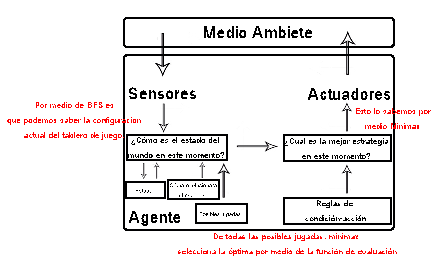
\includegraphics{agente-diagrama.pdf}
\caption{Diagrama en el cu\'al se describe al agente.}
\label{agente_modelos}
\end{figure}




% % % % % % % % % % % % % % % % % % % % % % % % % % % % % % % % % % % % % % % % % % % % % % % %
% % % % % % % % % % % % RISK ACOTADO % % % % % % % % % % % % % % % % % % % % % % % % % % % % % %
% % % % % % % % % % % % % % % % % % % % % % % % % % % % % % % % % % % % % % % % % % % % % % % % 
\section{Risk acotado.}

Tal y c\'omo se plantea en el juego original (\textbf{\textit{ve\'ase \cite{RISK}}}) el objetivo del juego continua siendo la dominaci\'on total de un territorio dado, de tal forma
que el juego queda concluido cu\'ando todos los territorios quedan bajo la dominaci\'on de 
un jugador.\\
En esta implementaci\'on acotaremos la cantidad de continentes, es decir, el desarrollo sera unicamente en un solo continente, tambi\'en la cantidad de dados se ve acotada a unicamente dos dados y restringido a dos jugadores.\\

Sin embargo mantendremos las dem\'as condiciones iniciales con respecto a las tropas y al equivalente de tropas en cada territorio, es decir:
\begin{list}{*}{}
\item Cada unidad representa una \textit{Armada}.
\item Cada \textit{Caballer\'ia} representa 5 unidades.
\item Cada \textit{Artiller\'ia} representa 10 unidades.
\end{list}

Teniendo ya esto definido, entonces, cada jugador tendr\'a un ejercito inicial de 3 tropas, por cada invasi\'on
se le asigna 3 tropas y por cada reforzamiento se le asigna 2 tropas.


\section{Marco te\'orico}

Para una posible implementaci\'on del juego de \textbf{RISK} hemos ideado una gr\'afica donde cada nodo
contiene como informaci\'on:
\begin{itemize}
 \item Nombre e identificador del pa\'is que se representa.
 \item Nombre e identificador del jugador que tiene invadido a este pa\'is, en caso de no estar invadido es nulo.
 \item N\'umero de tropas que tienen ocupado ese pa\'is, en caso de no estar invadido es cero.
\end{itemize}
Y cada arista representa la frontera de cada pa\'is.\\
Recomendamos utilizar la representaci\'on por lista de adyacencias, ya que la generaci\'on de movimientos y
la funci\'on de evaluaci\'on est\'an basados en el algoritmo \textit{BFS}, que es una b\'usqueda por amplitud.\\
Buscamos por amplitud ya que nuestro objetivo es lograr obtener todos los paises en el menor de movimientos, 
para esto necesitamos que el agente obtenga los paises con mayor n\'umero de vecinos, es decir, los v\'ertices
com mayor grado, para as\'i poder encapsular al enemigo.

\section{Generaci\'on de movimientos}

\subsection{Invasiones}

Por cada nodo existir\'a una nueva gr\'afica con el nuevo jugador y n\'umero de tropas asignado (3), lo
cual significa que habr\'a tantas nuevas gr\'aficas como n\'umero de v\'ertices que tenga el tablero; para
esto utilizaremos \textit{BFS}.

\begin{algorithm}
\begin{algorithmic}[1]
\REQUIRE Gr\'afica $G$ que representa el tablero actual,Jugador $actual$
\ENSURE Lista con todos los posibles invasiones
\STATE{$Queue$ $q$}
\STATE{$List invasiones$}
\STATE{$G^{\prime} = G$}
\FORALL{$v \in G$}
\STATE{$v.visitado = FALSE$}
\ENDFOR
\STATE{$v_{1}.visitado = FALSE$}\COMMENT{$v_{1}$ es el pa\'is con identificador 1}
\IF{$v_{1}.jugador = NULL$}
\STATE{$G^{\prime}.v_{1}.jugador = actual$}
\STATE{$G^{\prime}.v_{1}.tropas = 3$}
\STATE{$invasiones.add(G^{\prime})$}
\ENDIF
\STATE{$q.enqeue(v_{1})$}
\WHILE{$q.isNotEmpty()$}
\STATE{$v = q.remove()$}
\FORALL{$u \in Vecinos(v)$}
\IF{$u.visitado = FALSE$}
\STATE{$G^{\prime} = G$}
\IF{$v_{1}.jugador = NULL$}
\STATE{$G^{\prime}.u.jugador = actual$}
\STATE{$G^{\prime}.u.tropas = 3$}
\STATE{$invasiones.add(G^{\prime})$}
\ENDIF
\STATE{$u.visitado = TRUE$}
\STATE{$q.enqeue(u)$}
\ENDIF
\ENDFOR
\ENDWHILE
\RETURN $invasiones$
\end{algorithmic}
\caption{Definici\'on de la funci\'on $invasiones$}
\label{invasiones}
\end{algorithm}

\subsection{Reforzamientos}

Por cada nodo existir\'a una nueva gr\'afica con el nuevo n\'umero de tropas (2), lo
cual significa que habr\'a tantas nuevas gr\'aficas como paises pertenezcan a cada jugador; para
esto utilizaremos \textit{BFS}.

\begin{algorithm}
\begin{algorithmic}[1]
\REQUIRE Gr\'afica $G$ que representa el tablero actual
\ENSURE Lista con todos los posibles reforzamientos
\STATE{$Queue$ $q$}
\STATE{$List reforzamientos$}
\STATE{$G^{\prime} = G$}
\FORALL{$v \in G$}
\STATE{$v.visitado = FALSE$}
\ENDFOR
\STATE{$v_{1}.visitado = FALSE$}\COMMENT{$v_{1}$ es el pa\'is con identificador 1}
\IF{$G^{\prime}.v_{1}.jugador \neq NULL$}
\STATE{$G^{\prime}.v_{1}.tropas = v_{1}.tropas+2$}
\ENDIF
\STATE{$reforzamientos.add(G^{\prime})$}
\STATE{$q.enqeue(v_{1})$}
\WHILE{$q.isNotEmpty()$}
\STATE{$v = q.remove()$}
\FORALL{$u \in Vecinos(v)$}
\IF{$u.visitado = FALSE$}
\STATE{$G^{\prime} = G$}
\IF{$G^{\prime}.u.jugador \neq NULL$}
\STATE{$G^{\prime}.u.tropas = u.tropas+2$}
\STATE{$reforzamientos.add(G^{\prime})$}
\ENDIF
\STATE{$u.visitado = TRUE$}
\STATE{$q.enqeue(u)$}
\ENDIF
\ENDFOR
\ENDWHILE
\RETURN $reforzamientos$
\end{algorithmic}
\caption{Definici\'on de la funci\'on $reforzamientos$}
\label{reforzamientos}
\end{algorithm}

\subsection{Ataques}

Para cada nodo exisitir\'a nuevas gr\'aficas, una donde el ataque fue exitoso y se le asginar\'a una tropa donde
provino el ataque, y otra donde el ataque no fue existoso y se elimina el n\'umero de tropas con respecto al n\'umero
de tropas del atacado.

\begin{algorithm}
\begin{algorithmic}[1]
\REQUIRE Gr\'afica $G$ que representa el tablero actual, Jugador $actual$
\ENSURE Lista con todos los posibles ataques
\STATE{$Queue$ $q$}
\STATE{$List ataques$}
\FORALL{$v \in G$}
\STATE{$v.visitado = FALSE$}
\ENDFOR
\STATE{$v_{1}.visitado = FALSE$}\COMMENT{$v_{1}$ es el pa\'is con identificador 1}
\STATE{$q.enqeue(v_{1})$}
\WHILE{$q.isNotEmpty()$}
\STATE{$v = q.remove()$}
\FORALL{$u \in Vecinos(v)$}
\IF{$u.visitado = FALSE$}
\STATE{$G^{\prime} = G$}
\IF{$G^{\prime}.v.jugador = actual\ and\ G^{\prime}.u.jugador \neq NULL\ and\ G^{\prime}.u.jugador \neq actual$}
\IF{$G^{\prime}.v.tropas >= G^{\prime}.u.tropas$}
\STATE{$p = generaDados()$}\COMMENT{$generaDados()$ es una funci\'on 
que genera dos n\'umeros aleatorios y realiza su resta, representa los dados}
\IF{$p > 0$}
\STATE{$G^{\prime}.u.jugador = actual$}
\STATE{$G^{\prime}.u.tropas = 1$}
\STATE{$ataques.add(G^{\prime})$}
\ELSE
\STATE{$G^{\prime}.v.tropas = G^{\prime}.v.tropas - G^{\prime}.u.tropas$}
\STATE{$ataques.add(G^{\prime})$}
\ENDIF
\ENDIF
\ENDIF
\STATE{$u.visitado = TRUE$}
\STATE{$q.enqeue(u)$}
\ENDIF
\ENDFOR
\ENDWHILE
\RETURN $ataques$
\end{algorithmic}
\caption{Definici\'on de la funci\'on $ataques$}
\label{ataques}
\end{algorithm}

\section{Funci\'on de evaluaci\'on.}

La estrateg\'ia consiste en tomar cada pa\'is ocupado por \textbf{MAX} y ver a todos sus vecinos,
se sumar\'a el grado de cada v\'ertice y se resta los que pertenecen al oponente (esto para la parte de invasi\'on), acto seguido
se realiza una comparac\'ion de que paises son del oponente y cuanto se diferencian las tropas, para así tomar su
mejor desici\'on de ataque o reforzamiento.

$$ 
funcionEval(G)= \left\{\begin{array}{c l}
  \infty\ \textit{Max\ resulta\ ser\ ganador.}\\
  -\infty\ \textit{Min\ resulta\ ser\ ganador.}\\
  \mathtt{invadeReforzaAtaca(G)}\ \textit{e.o.c.}
\end{array}
\right.
$$

Donde:\\

$\mathtt{invadeReforzaAtaca}$ es un algoritmo que por medio de una modificaici\'on a \textit{BFS} cuenta
las tropas y paises de cada jugador, suma los grados de cada v\'ertice, suma los pertenecientes al jugador \textbf{MAX} 
y resta los del oponente \textbf{min}, tambi\'en por cada pa\'is de \textbf{MAX} resta los vecinos que pertenezcan 
a \textbf{min}, por otra parte bajo esa misma idea compara el n\'umero de tropas.\\

\begin{algorithm}
\begin{algorithmic}[1]
\REQUIRE La gr\'afica que representa el tablero
\ENSURE Es el entero descrito anteriormente
\STATE{$puntuacion = 0$}
\STATE{$Queue$ $q$}
\FORALL{$v \in G$}
\STATE{$v.visitado = FALSE$}
\ENDFOR
\COMMENT{$v_{1}$ es el pa\'is con identificador 1}
\STATE{$v_{1}.visitado = FALSE$}
\STATE{$q.enqeue(v_{1})$}
\WHILE{$q.isNotEmpty()$}
\STATE{$v = q.remove()$}
\FORALL{$u \in Vecinos(v)$}
\IF{$u.visitado = FALSE$}
\IF{$u.jugador = NULL\ and\ puntuacion < u.grado$}
\STATE{$puntuacion = puntuacion + u.grado$}
\ENDIF
\IF{$v.Jugador = MAX\ and\ Jugador = MIN$}
\STATE{$puntuacion = puntuacion - 1$}
\ENDIF
\IF{$u.jugador = MAX$}
\STATE{$puntuacion = puntuacion + u.daTropas() + 1$}
\ENDIF
\IF{$u.jugador = MIN$}
\STATE{$puntuacion = puntuacion - u.daTropas() - 1$}
\ENDIF
\IF{$v.Jugador = MAX\ and\ u.Jugador = MIN$}
\STATE{$puntuacion = puntuacion - 1$}
\ENDIF
\IF{$v.tropas > u.tropas$}
\STATE{$puntuacion = puntuacion + 1$}
\ENDIF
\IF{$v.tropas < u.tropas$}
\STATE{$puntuacion = puntuacion - 1$}
\ENDIF
\STATE{$u.visitado = TRUE$}
\STATE{$q.enqeue(u)$}
\ENDIF
\ENDFOR
\ENDWHILE
\RETURN $puntuacion$
\end{algorithmic}
\caption{Definici\'on de la funci\'on $invadeReforzaAtaca$}
\label{invadeReforzaAtaca}
\end{algorithm}

\section{Minimax}

Es un algoritmo para \textit{minimizar} la p\'erdida \textit{m\'axima} esperada en juegos de adversarios con
informaci\'on perfecta.\\

Como se mencion\'o anteriormente dado que el juego de \textbf{Risk} es pr\'acticamente intratable, se pierde esta propiedad
de informaci\'on perfecta, ya que el factor de ramificaci\'on es demasiado grande para poder ser implementada.\\

La idea te\'orica del algoritmo minimax es generar todo el \'arbol del juego, asignarles valor a cada
nodo del \'arbol y hacer un recorrido \textit{DFS} para obtener la mejor estrateg\'ia para \textbf{MAX}.\\

Dado que esto requiere una gran cantidad de espacio y tiempo, entonces la pr\'actica usual es realizar
el algoritmo \textit{minimax} de forma recursiva, tal que, vaya simulando la creaci\'on de las ramas y despu\'es
asginarles su valor y por \'ultimo obtener la mejor estrateg\'ia.\\
\newpage
\begin{algorithm}
\begin{algorithmic}[1]
\REQUIRE Entero $p$ que representa la profundiad del \'arbol, Jugador $actual$, gr\'afica $G$ que representa el tablero actual
\ENSURE  Gr\'afica que representa la mejor jugada
\STATE{$List\ movimientos$}
\IF{$graficaLlena(G)$}
\STATE{$movimientos = concatena(ataques(G,actual),reforzamientos(G))$}
\ELSE
\STATE{$movimientos = invasiones(G,actual)$}
\ENDIF
\STATE{$mejorPuntuacion = 0$}
\IF{$actual = 1$}
\STATE{$mejorPuntuacion = -\infty$}
\ELSE
\STATE{$mejorPuntuacion = \infty$}
\ENDIF
\STATE{$puntuacionActual = 0$}
\STATE{$mejorMovimiento = null$}
\IF{$movimientos.isEmpty()\ or\ profundidad = 0$}
\STATE{$mejorPuntuacion = funcionEval(G)$}
\STATE{$mejor = G$}
\ELSE
\FORALL{$movimiento \in movimientos$}
\IF{$actual = 1$}
\STATE{$puntuacionActual = funcionEval(minimax(p-1,min,G,f))$}
\IF{$puntuacionActual > mejorPuntuacion$}
\STATE{$mejorPuntuacion = puntuacionActual$}
\STATE{$mejor = movimiento$}
\ENDIF
\ELSE
\STATE{$puntuacionActual = funcionEval(minimax(p-1,max,G,f))$}
\IF{$puntuacionActual < mejorPuntuacion$}
\STATE{$mejorPuntuacion = puntuacionActual$}
\STATE{$mejor = movimiento$}
\ENDIF
\ENDIF
\ENDFOR
\ENDIF
\RETURN{$mejor$}
\end{algorithmic}
\caption{Definici\'on de $minimax$}
\label{minimax}
\end{algorithm}



\section{Complejidad.}

\textbf{Notacion}\\
$\nu$ denota a la cardinalidad del conjunto de v\'ertices \cite{bondy1976graph}.\\
$\epsilon$ denota a la cardinalidad del conjunto de aristas \cite{bondy1976graph}.\\

Procederemos a hacer el an\'alisis de complejidad para las funciones antes definidas, empecemos con la funci\'on \textbf{invaciones.}$^{\ref{invasiones}}$\\
\textit{Invaciones:}\\
En las primeras 3 lineas de c\'odigo es f\'acil observar que la complejidad es constante, por lo que obtenemos un $O(1)$.\\
Continuando con el an\'alisis observamos que asegurar el estado de \textit{"no visitado"} de cada nodo es de orden $O(n)$ pues eso se consigue visitando cada nodo en la gr\'afica.
Continuando as\'i en el ciclo \textit{while} y dado que \'este tiene contenido un ciclo \textit{for}, se observa que entonces la 
complejidad es del orden $O (\nu + \epsilon)$.\\

Con el algoritmo \textbf{Reforzamiento.}$^{\ref{reforzamientos} }$\\
\textit{Reforzamiento:}\\
El algoritmo de \textit{reforzamiento} tenemos que la secci\'on para visitar todos los nodos de la gr\'afica es de orden $O(n)$.
Continuamos con la secci\'on del ciclo \textit{while} y dado que dentro del \'este tiene un ciclo \textit{for} vemos nuevamente que tenemos una complejidad de $O(\nu + \epsilon)$.\\

Con el algoritmo \textbf{Ataques}$^{\ref{ataques} }$\\
Al ser un algoritmo basado \'unicamente en \textit{BFS}, de hecho, son s\'olo unas l\'ineas modificadas de este, su complejidad
corresponde al de dicho algoritmo, el m\'etodo $generaDados$ es de orden constante ya que generamos dos n\'umeros aleatorios
y se restan, todo esto es constante, por lo que el metodo $ataques$ tendr\'a una complejidad de $O(\nu + \epsilon)$.\\

Para el algoritmo \textbf{minimax}$^{\ref{ataques} }$\\
Sabemos que la complejidad del algoritmo \textit{minimax} es $O(b^{n})$ donde b es el factor de ramificaci\'on y n la profundidad del 
\'arbol \cite{russell2004inteligencia}, en nuestro caso habr\'a tantas ramas como la gr\'afica tiene v\'ertices y aristas debido
a todos los posibles reforzamientos, invasiones y ataques, 
por lo que la complejidad de \textit{minimax} en este caso es de $O((\nu+\epsilon)^{n})$ en el peor de los casos.

\section{Conclusiones.}
Se comenz\'o por una implementaci\'on en el lenguaje de programaci\'on \textit{JAVA} pero al momento de querer
realizar la lista de gr\'aficas de todos los posibles movimientos, se volvi\'o intratable en el sentido de que
generar tales gr\'aficas requiere de un gran espacio en memoria.\\
Acto seguido se opt\'o por pasar al lenguaje de programaci\'on \textit{Python} por su sencillez de la construcci\'on
de la gr\'afica que representa al tablero y sus funciones predefinidas sobre tal gr\'afica, pero  se tuvo el mismo
problema que \textit{JAVA}.\\
Implementar el juego de risk acotado, es posible, sin embargo a\'un con estas restricciones, es muy ineficiente para la
computadora, por la verificaci\'on de cada gr\'afica que representa a los movimientos.\\


% %Toda la bibliografía consultada debe de estar anexada en el archivo
% %referencias.bib 
\newpage

\bibliographystyle{plain}	
\nocite{*}
\bibliography{referencias.bib}{}


\end{document}
